\documentclass[a4paper,fleqn,12pt,twoside]{article}

\parindent=0pt
\parskip=2pt

\usepackage{amsfonts}	%% for \mathbb
\usepackage{bm}		%% bold math symbols
\usepackage{tikz}
\usepackage{placeins}
\usepackage{hyperref}

\newcommand\todo{\bigskip\fbox{TODO}\bigskip}

\newcommand{\hb}[2]{paragraph #2 on page #1 of the Handbook}
\newcommand{\hbm}[2]{{\marginpar{\scriptsize \sl Handbook #1, #2}}}

\newcommand\Arg{{\rm Arg}}
\newcommand\Log{{\rm Log}}
\newcommand\RE{{\rm Re}}
\newcommand\IM{{\rm Im}}

\newcommand\Complex{\mathbb{C}}
\newcommand\Integer{\mathbb{Z}}
\newcommand\Real{\mathbb{R}}

\title{Solutions to the M337/B 2013 exam paper}
\author{Edited by: Fred Youhanaie}
\date{12 June, 2013}

\begin{document}
\maketitle

\pagestyle{myheadings}
\markboth{M337/B 2013}{M337/B 2013}	% two sided
%%\markright{M337/B 2013}		% one sided

\section*{Copyright}

This work is licensed under a Creative Commons
Attribution-NonCommercial-ShareAlike 3.0 Unported License.

\newcommand\cclink{http://creativecommons.org/licenses/by-nc-sa/3.0/}
See the \href{\cclink}{by-nc-sa page}\footnote{\cclink} for details.

\section*{Solutions to Part I}
\subsection*{Solution 1}

\begin{itemize}
\item[(a)]

\begin{eqnarray*}
\exp(3+\frac{1}{4}\pi i)
	&=& e^3 \left( \cos \left(\frac{\pi}{4}\right) + i \sin \left(\frac{\pi}{4}\right) \right) \\
	&=& \frac{e^3}{\sqrt{2}} + i\frac{e^3}{\sqrt{2}}
\end{eqnarray*}

\item[(b)]
Let
\[ w^3 = -8 = 8( \cos\pi + i\sin\pi ) \]
then, \hbm{A1}{3.3}
\begin{eqnarray*}
w	&=& 8^\frac{1}{3} ( \cos ( \pi/3 ) + i \sin ( \pi/3 ) ) \\
	&=& 2 \left( \frac{1}{2} + i \frac{\sqrt{3}}{2} \right) \\
	&=& 1 + \sqrt{3}\,i
\end{eqnarray*}

\item[(c)]
Using the Pricinple $\alpha$th power:\hbm{A2}{5.3}
\begin{eqnarray*}
i^{1-2i}
	&=& \exp( (1-2i) \Log(i)) \\
	&=& \exp( (1-2i) (\log_e|i| + i\Arg(i) ) ) \\
	&=& \exp( i\pi/2 - 2i^2\pi/2 ) \\
	&=& \exp( \pi + i\pi/2 ) \\
	&=& e^\pi e^{i\pi/2} \\
	&=& e^\pi ( \cos(\pi/2) + i\sin(\pi/2) ) \\
	&=& ie^\pi
\end{eqnarray*}

\item[(d)]
Using the trigonometric functions\hbm{A2}{4.4}
\begin{eqnarray*}
\cos(i\log_e 2)
	&=& \frac{1}{2} \left( \exp(i^2\log_e 2) + \exp(-i^2\log_e 2) \right) \\
	&=& \frac{1}{2} \left( \exp(-\log_e 2) + \exp(\log_e 2) \right) \\
	&=& \frac{1}{2} \left( 1/2 + 2 \right) \\
	&=& \frac{5}{4}
\end{eqnarray*}

\end{itemize}


\newpage
\subsection*{Solution 2}

\begin{itemize}
\item[(a)][DC]

Below are the sketches of the four sets:

%
%	This is the original file provided by Dominic Corbett on the
%	M337 Forum so that it could be included in the solutions paper.
%
\documentclass[10pt,a4paper]{article}
\usepackage{amsmath}
\usepackage{amsfonts}
\usepackage{amssymb}
\DeclareMathOperator{\re}{Re}
\DeclareMathOperator{\im}{Im}
\usepackage{fullpage}
\delimitershortfall-1sp
\newcommand{\cbr}[1]{\left\{#1\right\}}
\newcommand{\abs}[1]{\left\lvert#1\right\rvert}
\usepackage{lastpage}
\usepackage{tikz}
\usepackage{subcaption}
\usepackage{fancyhdr}
\pagestyle{fancy}
\lhead{M337 --- 2013 Exam Solutions}
\chead{}
\rhead{DBJC}
\headsep = 10pt
\lfoot{}
\cfoot{\thepage\ of \pageref{LastPage}}
\rfoot{}
\renewcommand{\headheight}{12.0pt}
\renewcommand{\headrulewidth}{0.4pt}
\renewcommand{\footrulewidth}{0.4pt}
\definecolor{light-gray}{gray}{0.75}
\definecolor{light-light-gray}{gray}{0.875}
\usepackage{xr-hyper}
\usepackage[bookmarks=true,backref=section,colorlinks=true,linkcolor=black,pdftitle={M337 2013 Exam Solutions},pdfauthor={DBJC}]{hyperref}
\begin{document}
\begin{figure}
	\centering
	\begin{subfigure}{0.49\textwidth}
		\centering
		\begin{tikzpicture}[scale=0.65][font=\scriptsize]
			\foreach \x in {-5,-4,-3,-2,-1,1,2,3,4,5}{							% reference grid
				\foreach \y in {-5,-4,-3,-2,-1,1,2,3,4,5}{
					\filldraw [light-gray] (\x,\y) circle (0.5pt) ;
				}
			}
			\draw [draw=black,fill=light-light-gray] (0,0) circle (4);					% outer limit
			\draw [draw=black,dashed,fill=white] (-0,0) circle (1);					% inner limit
			\node[font=\normalsize] at (1.5,2) {$ A $};							% label
			\draw [-latex] (-5.5,0) -- (5.5,0) node [above]  {$\re\{z\}$};				% Real axis
			\draw [-latex] (0,-5.5) -- (0,5.5) node [right] {$\im\{z\}$};				% Imaginary axis
			\foreach \n in {-5,-4,...,-1,1,2,...,4,5}{								% real axis ticks
				\draw (\n,-1pt) -- (\n,1pt)   node [below] {$\n$};
			}
			\foreach \n in {-5,-4,...,-1,1,2,...,4,5}{								% imaginary axis ticks
				\draw (-1pt,\n) -- (1pt,\n)   node [left] {$\n$};
			}
		\end{tikzpicture}
		\caption{Sketch of the set $ A = \cbr{ z : 1 < \abs{ z } \leq 4 } $.}
		\label{setA}
	\end{subfigure}
	\begin{subfigure}{0.49\textwidth}
		\centering
		\begin{tikzpicture}[scale=0.65][font=\scriptsize]
			\foreach \x in {-5,-4,-3,-2,-1,1,2,3,4,5}{							% reference grid
				\foreach \y in {-5,-4,-3,-2,-1,1,2,3,4,5}{
					\filldraw [light-gray] (\x,\y) circle (0.5pt) ;
				}
			}
			\begin{scope}
				\clip (-2.5,-2.5) rectangle (5.5,5.5);
				\filldraw [dashed,fill=light-light-gray] (-1,-1) rectangle (6,6);		% excluded boundaries
			\end{scope}
			\node[font=\normalsize] at (2.5,2.5) {$ B $};							% label
			\draw [-latex] (-5.5,0) -- (5.5,0) node [above]  {$\re\{z\}$};				% Real axis
			\draw [-latex] (0,-5.5) -- (0,5.5) node [right] {$\im\{z\}$};				% Imaginary axis
			\foreach \n in {-5,-4,...,-1,1,2,...,4,5}{								% real axis ticks
				\draw (\n,-1pt) -- (\n,1pt)   node [below] {$\n$};
			}
			\foreach \n in {-5,-4,...,-1,1,2,...,4,5}{								% imaginary axis ticks
				\draw (-1pt,\n) -- (1pt,\n)   node [above=0.3mm, left] {$\n$};
			}
		\end{tikzpicture}
		\caption{Sketch of the set $ B = \cbr{ z : \re z > -1 , \im z > -1 } $.}
		\label{setB}
	\end{subfigure}
	\begin{subfigure}{0.49\textwidth}
		\centering
		\begin{tikzpicture}[scale=0.65][font=\scriptsize]
			\foreach \x in {-5,-4,-3,-2,-1,1,2,3,4,5}{							% reference grid
				\foreach \y in {-5,-4,-3,-2,-1,1,2,3,4,5}{
					\filldraw [light-gray] (\x,\y) circle (0.5pt) ;
				}
			}
			\begin{scope}
				\clip (-5,-5) -- (-5,5) -- (-1,5) -- (-1,-1) -- (5,-1) -- (5,-5) -- cycle;
				\draw [draw=black,fill=light-light-gray] (0,0) circle (4);				% outer limit
			\end{scope}
			\begin{scope}
				\clip (0,0) circle (4);
				\draw (-1,5) -- (-1,-1) -- (5,-1);								% new boundaries
			\end{scope}
			\node[font=\normalsize] at (-2.5,1.5) {$ C $};						% label
			\draw [-latex] (-5.5,0) -- (5.5,0) node [above]  {$\re\{z\}$};				% Real axis
			\draw [-latex] (0,-5.5) -- (0,5.5) node [right] {$\im\{z\}$};				% Imaginary axis
			\foreach \n in {-5,-4,...,-1,1,2,...,4,5}{								% real axis ticks
				\draw (\n,-1pt) -- (\n,1pt)   node [below] {$\n$};
			}
			\foreach \n in {-5,-4,...,-1,1,2,...,4,5}{								% imaginary axis ticks
				\draw (-1pt,\n) -- (1pt,\n)   node [above=0.3mm, left] {$\n$};
			}
			\filldraw [fill=white] (-1,0) circle (2pt);								% excluded points
			\filldraw [fill=white] (0,-1) circle (2pt);
		\end{tikzpicture}
		\caption{Sketch of the set $ C = A - B $.}
		\label{setC}
	\end{subfigure}
	\begin{subfigure}{0.49\textwidth}
		\centering
		\begin{tikzpicture}[scale=0.65][font=\scriptsize]
			\foreach \x in {-5,-4,-3,-2,-1,1,2,3,4,5}{							% reference grid
				\foreach \y in {-5,-4,-3,-2,-1,1,2,3,4,5}{
					\filldraw [light-gray] (\x,\y) circle (0.5pt) ;
				}
			}
			\draw (-1,5.5) -- (-1,-1) -- (5.5,-1);								% boundary
			\node[font=\normalsize] at (-1.5,1.75) {$ D $};						% label
			\draw [-latex] (-5.5,0) -- (5.5,0) node [above]  {$\re\{z\}$};				% Real axis
			\draw [-latex] (0,-5.5) -- (0,5.5) node [right] {$\im\{z\}$};				% Imaginary axis
			\foreach \n in {-5,-4,...,-1,1,2,...,4,5}{								% real axis ticks
				\draw (\n,-1pt) -- (\n,1pt)   node [below] {$\n$};
			}
			\foreach \n in {-5,-4,...,-1,1,2,...,4,5}{								% imaginary axis ticks
				\draw (-1pt,\n) -- (1pt,\n)   node [above=0.3mm, left] {$\n$};
			}
		\end{tikzpicture}
		\caption{Sketch of the set $ D = \partial D $.}
		\label{setD}
	\end{subfigure}
	\caption{Sketches of the sets $ A $, $ B $, $ C $, and $ D $.}
	\label{2aSketches}
\end{figure}
\end{document}


\item[(b)]
\begin{itemize}
\item[(i)][FY,LK]

\begin{itemize}
\item[$A$] is not a region, not open
\item[$B$] is a region
\item[$C$] is not a region, not open
\item[$D$] is not a region, not open
\end{itemize}

\item[(ii)]

\begin{itemize}
\item[$A$] is not compact, not closed
\item[$B$] is not compact, not closed
\item[$C$] is not compact, not closed
\item[$D$] is not compact, not bounded
\end{itemize}

\end{itemize}

\end{itemize}


\newpage
\subsection*{Solution 3}

\begin{itemize}
\item[(a)]
By definition \hbm{A2}{2.3}
\[ \Gamma: \gamma(t) = 2(\cos(t) + i\sin(t)) = 2e^{it},\;\; (t\in[0,2\pi]) \]

\item[(b)]
We use the polar form from above,
\begin{eqnarray*}
\overline{\gamma(t)}
	&=& 2e^{-it}\\
\\
\gamma'(t)
	&=& 2ie^{it}
\end{eqnarray*}
So,\hbm{B1}{2.1}
\begin{eqnarray*}
\int_\Gamma \overline{z}\,dz
	&=& \int_0^{2\pi} \left( 2e^{-it} 2ie^{it} \right) \, dt \\
	&=& \int_0^{2\pi} 4i\,dt \\
	&=& \left[ 4it \right]_0^{2\pi} \\
	&=& 8\pi i
\end{eqnarray*}

\item[(c)][FY,LK]
Let
\[ f(z) = \frac{ 2\sin z }{ \overline{z}^2+1 } \]
then, $f$ is continuous on $\Gamma$ by combination rules, where $\Gamma$
has length $L=4\pi$


So, using the triangle inequality\hbm{A1}{5.2(a)}
\begin{eqnarray*}
|2\sin z|
	&=& \left| 2\frac{1}{2i} \left( e^{iz} - e^{-iz} \right) \right| \\
	&=& \left| -i \left( e^{iz} - e^{-iz} \right) \right| \\
	&\le& \left| e^{iz} \right| + \left| e^{-iz} \right| \\
	&=& e^{\RE\,z} + e^{-\RE\,z} \\
	&<& 2e^2
\end{eqnarray*}
%%
And, using the backward triangle inequality\hbm{A1}{5.2(b)}
\begin{eqnarray*}
\left| \overline{z}^2+1 \right|
	&\ge& \left| |z|^2 - |1| \right| \\
	&=& |4-1| \\
	&=& 3
\end{eqnarray*}
%%
So,
\begin{eqnarray*}
|f(z)|	&=& \left| \frac{ 2\sin z }{ \overline{z}^2+1 } \right| \\
	&=& \frac{ |2\sin z| }{ \left| \overline{z}^2+1 \right| } \\
	&\le& \frac{2e^2}{3} \\
	&=& M
\end{eqnarray*}
%%
then by the Estimation Theorem.\hbm{B1}{4.3}
\[
\left| \int_\Gamma \frac{ 2\sin z }{ \overline{z}^2+1 }\,dz \right|
\le ML = \frac{2e^2}{3} 4\pi = \frac{8\pi e^2}{3} 
\]

\end{itemize}


\newpage
\subsection*{Solution 4}

\begin{itemize}
\item[(a)]

Let $R=\{ z: |z|<2 \}$, and $f(z)=\frac{\Log(2-z)}{z^2+4}$, then
\begin{enumerate}
\item $R$ is a simply-connected region
\item $f$ is analytic on $R$
\item $C$ is a closed contour in $R$
\end{enumerate}
Hence, by Cauchy's Theorem\hbm{B2}{1.4}
\[
\int_C \frac{\Log(2-z)}{z^2+4}\,dz = 0
\]

\item[(b)]

Let $R=\{ z: |z|<2 \}$, and $f(z)=\frac{\Log(2-z)}{z-2}$, then
\begin{enumerate}
\item $R$ is a simply-connected region
\item $f$ is analytic on $R$
\item $C$ is a simple-closed contour in $R$
\item $z=0$ is inside $C$
\end{enumerate}
Hence, by Cauchy's Integral Formula \hbm{B2}{2.1}
\begin{eqnarray*}
f(0)	&=& \frac{1}{2\pi i} \int_C \frac{f(z)}{z}\, dz \\
	&=& \frac{1}{2\pi i} \int_C \frac{\Log(2-z)/(z-2)}{z}\, dz \\
\end{eqnarray*}
where,
\[ f(0) = \Log(2)/(-2) = -\log_e 2/2 \]

\[
\int_C \frac{\Log(2-z)}{z(z-2)}\,dz = -\frac{\log_e 2}{2}\times2\pi i = -\pi\log_e 2\,i
\]

\item[(c)][FY,JK]

Let $R=\{ z: |z|<2 \}$, and $f(z)=\Log(2-z)$, then
\begin{enumerate}
\item $R$ is a simply-connected region
\item $f$ is analytic on $R$
\item $C$ is a simple-closed contour in $R$
\item $z=0$ is inside $C$
\item $f$ is differentiable at $z=0$
\end{enumerate}
Hence, by Cauchy's 2nd Derivative Formula\hbm{B2}{3.1}
\begin{eqnarray*}
f^{(2)}(0)
	&=& \frac{2!}{2\pi i} \int_C \frac{ f(z) }{ z^3 }\, dz \\
	&=& \frac{1}{\pi i} \int_C \frac{ \Log(2-z) }{ z^3 }\, dz
\end{eqnarray*}
where,
\begin{eqnarray*}
f'(z)	&=& -\frac{1}{2-z} \\
f^{(2)}(z)
	&=& -\frac{1}{(2-z)^2}
\end{eqnarray*}
So,
\[
\int_C \frac{ \Log(2-z) }{ z^3 }\,dz = f^{(2)}(0)\pi i = -\frac{\pi i}{4}
\]

\end{itemize}


\newpage
\subsection*{Solution 5}

\begin{itemize}
\item[(a)]
\todo
\item[(b)]
\todo
\end{itemize}


\newpage
\subsection*{Solution 6}

\begin{itemize}
\item[(a)]
\todo
\item[(b)]
\todo
\end{itemize}


\newpage
\subsection*{Solution 7}

\begin{itemize}
\item[(a)]

$q$ is continuous on $\Complex$, and its conjugate
$\overline{q}(z) = z+1+i$
is entire, hence $q$ is a model fluid flow.\hbm{D2}{1.14}

\item[(b)]

The complex potential function, $\Omega(z)$ for $q$ is a primitive of
$\overline{q}$, so
\[
\Omega(z) = \frac{z^2}{2}+(1+i)z
\]
Now, for $z=x+iy$
\begin{eqnarray*}
\Omega(x+iy)
	&=& \frac{ (x+iy)^2 }{ 2 } + (1+i)(x+iy) \\
	&=& \frac{ x^2-y^2 +2xyi }{2} + x + iy + ix - y \\
	&=& x^2/2 - y^2/2 + x - y + i(x + y + xy) \\
	&=& \Phi(x,y) + i\Psi(x,y)
\end{eqnarray*}
So, $q$ has streamline $\Psi(x,y)=x+y+xy=C$, for constant $C$.\hbm{D2}{2.1}

For the streamline through the point 1, $\Psi(1,0) = 1$, so, the
streamline through point 1 has the equation $x+y+xy=1$, a hyperbola.

\todo

\item[(c)]

\todo

\end{itemize}


\newpage
\subsection*{Solution 8}

\begin{itemize}
\item[(a)]

The iteration sequence
\[
z_{n+1} = 15z_n^2 + 3z_n + \frac{1}{16}
\]
is conjugate to the iteration sequence\hbm{D3}{2.1}
\[
w_{n+1} = w_n+d
\]
where
\[
d = \frac{15}{16} + \frac{3}{2} - \frac{9}{4} = \frac{15+24-36}{16} = \frac{3}{16}
\]
so, $w_{n+1} = w_n+\frac{3}{16}$.
The conjugating function is
\[
h(z) = 15z+\frac{1}{2}\times3 = 15z+\frac{3}{2}
\]
So, $w_0 = h(z_0) = h(0) = 0+\frac{3}{2} = \frac{3}{2}$

\item[(b)]

$P_{\frac{3}{16}}$ has fixed points at $z$, where $z^2+\frac{3}{16}=z$, these are the solutions to the equation
\[
z^2-z+\frac{3}{16}
\]
So
\[
z = \frac{ 1 \pm \sqrt{1 - 12/16} }{ 2 } = \frac{ 1 \pm \sqrt{1/4} }{ 2 } = \frac{1}{2}\pm\frac{1}{4}
\]
Hence, the fixed points of $P_{\frac{3}{16}}$ are $\frac{3}{4}$ and $\frac{1}{4}$.

Now, $P'_{\frac{3}{16}}(z) = 2z$, so
\[ \left|P'_{\frac{3}{16}}\left(\frac{3}{4}\right)\right| = \frac{6}{4} = \frac{3}{2} > 1 \]
and
\[ \left|P'_{\frac{3}{16}}\left(\frac{1}{4}\right)\right| = \frac{2}{4} = \frac{1}{2} < 1 \]
Hence, $\frac{1}{4}$ is an attracting fixed point and $\frac{3}{4}$ is a repelling one.

\item[(c)]

Let $c=-\frac{3}{2}+i$, then it appears from the diagram that $c$ is
outside the Mandelbrot set.\hbm{D3}{4.3}

Using the specificion for $M$\hbm{D3}{4.5}
\[
|P_c(0)| = |-3/2+i| = \sqrt{9/4+1} = \sqrt{13/4} < 2
\]
We go for the next iteration:
\begin{eqnarray*}
|P_c^{(2)}(0)|
	&=& |(-3/2+i)^2-3/2+i| \\
	&=& |9/4-1-3i-3/2+i| \\
	&=& |-1/4-2i| \\
	&=& \sqrt{1/16+4} \\
	&=& \sqrt{65/4} \\
	&\simeq& 4.0 > 2
\end{eqnarray*}
Hence, $c$ lies outside the Mandelbrot set, $c\not\in M$.

\end{itemize}


\newpage

\section*{Solutions to Part II}
\subsection*{Solution 9}

\begin{itemize}
\item[(a)]

\begin{itemize}
\item[(i)]

Let $z=x+iy$, then
\begin{eqnarray*}
f(x+iy)	&=& (x+iy)(3+\overline{x+iy}) + \RE (x+iy) \\
	&=& 3(x+iy) + x^2 + y^2 + x \\
	&=& x^2+y^2+4x + i3y \\
	&=& u(x,y) + iv(x,y)
\end{eqnarray*}
where, $u(x,y) = x^2+y^2+4x$ and $v(x,y) = 3y$.

\item[(ii)]

The function $f$ is defined on $\Complex$. For $u$ and $v$, we have
\[
\begin{array}{ll}
\frac{\partial u}{\partial x} = 2x+4
	& \frac{\partial v}{\partial x} = 0 \\
\\
\frac{\partial u}{\partial y} = 2y
	& \frac{\partial v}{\partial y} = 3
\end{array}
\]
The Cauchy-Riemann equations for the above partial derivatives hold when
$x=-\frac{1}{2}$ and $y=0$.\hbm{A4}{2.1}

Now, $\alpha=\left(-\frac{1}{2},0\right)$, as $f$ is defined on $\Complex$ and the
partial derivatives for $u$ and $v$:
\begin{enumerate}
\item exist on $\Complex$
\item are continuous at $\alpha$
\item satisfy the Cauchy-Riemann equations at $\alpha$
\end{enumerate}
then, by the Cauchy-Riemann Converse Theorem,\hbm{A4}{2.3} $f$ is
differentiable at $\alpha$.

Since $f$ is only differentiable at $\alpha$, then there is no region
where $f$ is analytic and contains $\alpha$, hence $f$ is not analytic
at $\left(-\frac{1}{2},0\right)$.\hbm{A4}{1.3}

\item[(iii)]

From the Cauchy-Riemann Converse Theorem:\hbm{A4}{2.3}
\begin{eqnarray*}
f'\left(-\frac{1}{2}\right)
	&=& \frac{\partial u}{\partial x}\left(-\frac{1}{2},0\right)
		+ i\frac{\partial v}{\partial x}\left(-\frac{1}{2},0\right) \\
	&=& 2\left(-\frac{1}{2}\right) + 4 + i0 \\
	&=& 3
\end{eqnarray*}

\end{itemize}

\item[(b)]

\begin{itemize}
\item[(i)]

Since $g$ is analytic on $\Complex-\{0\}$, with $g'(z) = 1-\frac{i}{z^2}$,
and, since $g'(1)=1-i\ne0$, then $g$ is conformal at $1$.\hbm{A4}{4.6}

\item[(ii)]

With $g(1)=1+i$, $|g'(1)|=|1-i|=\sqrt{2}$ and
$\Arg(g'(1))=-\frac{\pi}{4}$,
the effect of $g$ on a small disc centred at $1$ is to move it to $1+i$,
scale it by $\sqrt{2}$ and rotate it by $\frac{\pi}{4}$ clockwise.\hbm{A4}{1.11}

\item[(iii)]

Since, $\gamma_1(0) = e^{i0} = 1$ and $\gamma_2(1) = (1-1)i+1 = 1$,
then $\gamma_1$ and $\gamma_2$ meet at $t=0$ and $t=1$ respectively.

Let $\theta$ be the angle from $\Gamma_1$ to $\Gamma_2$ at $1$,
then\footnote{From FY's copy of the handbook!}
\hbm{A4}{1.12}
\[
\theta	= \Arg \left( \frac{ \gamma_2'(1) }{ \gamma_1'(0) } \right)
	= \Arg \left( \frac{ ie^{i0} }{ 1+i } \right)
	= \Arg \left( \frac{1}{2} + \frac{i}{2} \right)
	= \frac{\pi}{4}
\]
Hence, at the point of intersection, the angle from $\Gamma_1$ to
$\Gamma_2$ is $\frac{\pi}{4}$.

\item[(iv)]

The paths are shown below:


%
%	Sketches for Q9(b)(iv)
%
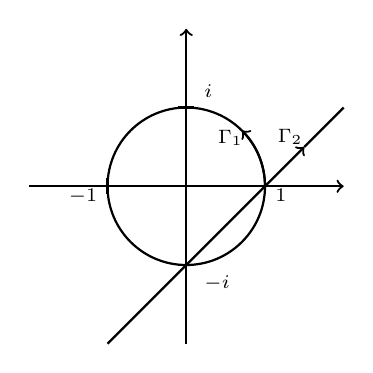
\begin{tikzpicture}
	% grid for draft only
	%%\draw [help lines] (-2,-2) grid (2,2);
	% the X-axis
	\draw[->,thick] (-2,0)--(2,0);
	\draw[thick] (-1,-0.1) -- (-1,0.1) node[below left] {\scriptsize $-1$};
	\draw[thick] (1,-0.1) -- (1,0.1) node[below right] {\scriptsize $1$};
	% the Y-axis
	\draw[->,thick] (0,-2)--(0,2);
	\draw[thick] (-0.1,-1) -- (0.1,-1) node[below right] {\scriptsize $-i$};
	\draw[thick] (-0.1,1) -- (0.1,1) node[above right] {\scriptsize $i$};
	% \Gamma_1
	\draw[thick] (0,0) circle (1);
	\draw[->,thick] (1,0) arc (0:45:1) node[below left=-4pt] {\scriptsize $\Gamma_1$};
	% \Gamma_2
	\draw[->,thick] (-1,-2) -- (1.5,0.5) node[above left=-3pt] {\scriptsize $\Gamma_2$};
	\draw[thick] (1.5,0.5) -- (2,1);
\end{tikzpicture}



\item[(v)]

The directions of $g(\Gamma_1)$ and $g(\Gamma_2)$ are shown below:


%
%	Sketches for Q9(b)(v)
%
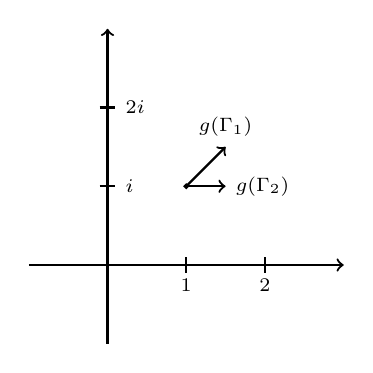
\begin{tikzpicture}
	% grid for draft only
	%%\draw [help lines] (-1,-1) grid (3,3);
	% the X-axis
	\draw[->,thick] (-1,0)--(3,0);
	\draw[thick] (1,-0.1) -- (1,0.1) node[below=4pt] {\scriptsize $1$};
	\draw[thick] (2,-0.1) -- (2,0.1) node[below=4pt] {\scriptsize $2$};
	% the Y-axis
	\draw[->,thick] (0,-1)--(0,3);
	\draw[thick] (-0.1,1) -- (0.1,1) node[right] {\scriptsize $i$};
	\draw[thick] (-0.1,2) -- (0.1,2) node[right] {\scriptsize $2i$};
	% little dot at g(1)
	\draw[thick] (1,1) circle(0.02);
	% g(\Gamma_1)
	\draw[->,thick] (1,1) -- (1.5,1.5) node[above] {\scriptsize $g(\Gamma_1)$};
	% g(\Gamma_2)
	\draw[->,thick] (1,1) -- (1.5,1) node[right] {\scriptsize $g(\Gamma_2)$};
\end{tikzpicture}



\item[(vi)][DC,FY]

The image of the unit circle, $\Gamma(t)=e^{it}$ for $t\in[0,2\pi]$,
under $g$ is as follows:\hbm{A2}{2.5}
\begin{eqnarray*}
g(\Gamma(t))
	&=& g(e^{it}) \\
	&=& e^{it}+ie^{-it} \\
	&=& \cos(t) + i\sin(t) +i(\cos(-t)+i\sin(-t)) \\
	&=& \cos(t)+i\sin(t)+i\cos(t)-i^2\sin(t) \\
	&=& (\cos(t)+\sin(t))(1+i)
\end{eqnarray*}

\end{itemize}

\end{itemize}


\newpage
\subsection*{Solution 10}

\begin{itemize}
\item[(a)]

\begin{itemize}

\item[(i)]

The function $f(z)$ has two simple poles at $z=1$ and $z=5$.

\item[(ii)]

A sketch of the annulus is shown below:

%
%	Sketches for Q10(a)(i)

%
%	The annulus {z: 1 < |z-2| < 3}
%
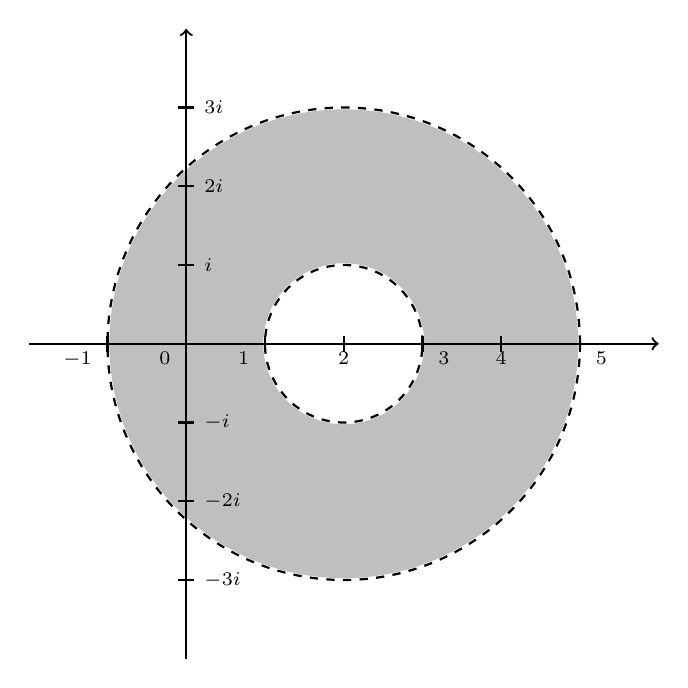
\begin{tikzpicture}
	% shading - must be drawn before the rest!
	\filldraw[even odd rule,color=lightgray] (2,0) circle(2.97) (2,0) circle(1.03);
	% grid for draft only
	%%\draw [help lines] (-2,-4) grid (6,4);
	% the X-axis
	\draw[->,thick] (-2,0)--(6,0);
	\foreach \x in {-1, 0, 1} {
		\draw[thick] (\x,-0.1) -- (\x,0.1) node[below left=2pt] {\scriptsize $\x$};
	}
	\foreach \x in {2, 4} {
		\draw[thick] (\x,-0.1) -- (\x,0.1) node[below=2pt] {\scriptsize $\x$};
	}
	\foreach \x in {3, 5} {
		\draw[thick] (\x,-0.1) -- (\x,0.1) node[below right=2pt] {\scriptsize $\x$};
	}
	% the Y-axis
	\draw[->,thick] (0,-4)--(0,4);
	\foreach \y in {2, 3} {
		\draw[thick] (-0.1,-\y) -- ( 0.1,-\y) node[right] {\scriptsize $-\y i$};
		\draw[thick] (-0.1, \y) -- ( 0.1, \y) node[right] {\scriptsize $ \y i$};
	}
	\draw[thick] (-0.1,-1) -- (0.1,-1) node[right] {\scriptsize $-i$};
	\draw[thick] (-0.1, 1) -- (0.1, 1) node[right] {\scriptsize $ i$};
	% inner circle border
	\draw[thick,style=dashed] (2,0) circle (1);
	% outer circle border
	\draw[thick,style=dashed] (2,0) circle (3);
\end{tikzpicture}



\todo
\end{itemize}

\item[(b)]

\begin{itemize}
\item[(i)]
\todo
\item[(ii)]
\todo
\end{itemize}

\end{itemize}


\newpage
%
%	This is the modified solution for Q11 supplied by Dominic Corbett
%
\subsection*{Solution 11}

\begin{itemize}

\item[(a)][DC]

Note that
\begin{align*}
	f ( z )
	&=
	\frac{ \pi \cos ( \pi z ) }{ \del{ 4 z + 3 i } \del{ 4 z - 3 i } \sin ( \pi z ) }
\intertext{so by the cover-up rule (\textit{HB28---1.3})}
	\Res ( f , - i \tfrac{3}{4} )
	&=
	\frac{ \pi \cos ( - \pi i \tfrac{3}{4} ) }{ 4 \del{ 4 ( - i \tfrac{3}{4} ) - 3 i } \sin ( - \pi i \tfrac{3}{4} ) }
	\\
	&=
	\frac{ \pi \cosh ( - \tfrac{3}{4} \pi ) }{ - 24 i^2 \sinh ( - \tfrac{3}{4} \pi ) }
	\\
	&=
	\underline{\underline{
	- \tfrac{ \pi }{ 24 } \coth ( \tfrac{3}{4} \pi )
	}}
\intertext{and}
	\Res ( f , i \tfrac{3}{4} )
	&=
	\frac{ \pi \cos ( \pi i \tfrac{3}{4} ) }{ 4 \del{ 4 ( i \tfrac{3}{4} ) + 3 i } \sin ( \pi i \tfrac{3}{4} ) }
	\\
	&=
	\frac{ \pi \cosh ( \tfrac{3}{4} \pi ) }{ 24 i^2 \sinh ( \tfrac{3}{4} \pi ) }
	\\
	&=
	\underline{\underline{
	- \tfrac{ \pi }{ 24 } \coth ( \tfrac{3}{4} \pi )
	}}
\intertext{and by the $ g/h $ rule (\textit{HB28---1.2})}
	\Res ( f , 0 )
	&=
	\frac{ \pi \cos ( \pi (0) ) }{ \del{ 4 (0) + 3 i } \del{ 4 (0) - 3 i } \pi \cos ( \pi (0) ) }
	\\
	&=
	\frac{ 1 }{ ( 3 i ) ( - 3 i ) }
	\\
	&=
	\underline{\underline{
	\tfrac{ 1 }{ 9 }
	}}
\end{align*}

\item[(b)][DC]

$ \phi ( n ) = \frac{1}{16 n^2 + 9} $ is an even function which is analytic on $ \Complex $ except for poles at the points $ \tfrac{3}{4} i $ and $ - \tfrac{3}{4} i $. Now, if $ S_N $ is the square contour with vertices at $ (N + \tfrac{1}{2})(\pm 1 \pm i) $, then its length is $ L = 4 ( 2 N + 1 ) $ and
\label{11b}
\begin{align*}
	\abs{\cot \pi z}
	&\leq
	2
	\;\;\;\text{for $ z \in S_N $ (\textit{HB30---4.2})}
\intertext{and since $ \abs{ z } \geq N + \frac{1}{2} $ for $ z \in S_N $, we have}
	\abs{ 16 z^2 + 9 }
	&\geq
	\abs{ \abs{ 16 z^2 } - \abs{ 9 } }
	\;\;\;(\textit{HB11---5.2})
	\\
	&=
	\abs{ 16 \abs{ z }^2 - 9 }
	\\
	&\geq
	\abs{ 16 ( N + \tfrac{1}{2} )^2 - 9 }
	\;\;\;\text{for $ z \in S_N $}
	\\
	\therefore
	\abs{ f ( z ) }
	=
	\abs{ \frac{ \pi \cot ( \pi z ) }{ 16 z^2 + 9 } }
	&\leq
	\frac{ 2 \pi }{ 16 ( N + \tfrac{1}{2} )^2 - 9 }
	=
	M
	\;\;\;\text{for $ z \in S_N $}
\intertext{Hence, by the Estimation Theorem,}
	\abs{ \int_{S_N} f ( z ) \dd z }
	&\leq
	\frac{ 2 \pi }{ 16 ( N + \tfrac{1}{2} )^2 - 9 } \cdot 4 ( 2 N + 1 ) ,
\intertext{which tends to $ 0 $ as $ N \to \infty $, that is}
	\lim_{N\to\infty} \int_{S_N} f ( z ) \dd z
	&=
	0
\intertext{It follows by \textit{HB30---4.1} that}
	\sum_{n=1}^\infty \frac{1}{16 n^2 + 9}
	&=
	- \tfrac{1}{2} \del{ \Res ( f , 0 ) + \Res ( f , - i \tfrac{3}{4} ) + \Res ( f , i \tfrac{3}{4} ) }
	\\
	&=
	- \tfrac{1}{2} \del{ \tfrac{ 1 }{ 9 } - \tfrac{ \pi }{ 24 } \coth ( \tfrac{3}{4} \pi ) - \tfrac{ \pi }{ 24 } \coth ( \tfrac{3}{4} \pi ) }
	\\
	&=
	\underline{\underline{
	\tfrac{ \pi }{ 24 } \coth ( \tfrac{3}{4} \pi ) - \tfrac{1}{18}
	}}
\end{align*}

\item[(c)][DC]

Since
\begin{align*}
	\sum_{n=-\infty}^\infty \frac{1}{16 n^2 + 9}
	&=
	\sum_{n=-\infty}^{-1} \frac{1}{16 n^2 + 9}
	+
	\frac{1}{16 (0)^2 + 9}
	+
	\sum_{n=1}^\infty \frac{1}{16 n^2 + 9}
	\\
	&=
	\sum_{n=\infty}^{1} \frac{1}{16 (-n)^2 + 9}
	+
	\frac{1}{9}
	+
	\sum_{n=1}^\infty \frac{1}{16 n^2 + 9}
	\\
	&=
	\frac{1}{9}
	+
	2 \sum_{n=1}^\infty \frac{1}{16 n^2 + 9}
	\;\;\hbox{(sum of positive reals indp't of order)}
\intertext{we can simply substitute in our result from part~(b) to give}
	\sum_{n=-\infty}^\infty \frac{1}{16 n^2 + 9}
	&=
	\frac{1}{9}
	+
	\tfrac{ 2 \pi }{ 24 } \coth ( \tfrac{3}{4} \pi ) - \tfrac{2}{18}
	\\
	&=
	\underline{\underline{
	\tfrac{ \pi }{ 12 } \coth ( \tfrac{3}{4} \pi )
	}}
	\;\;\;\textsc{qed}
\end{align*}

\end{itemize}

\newpage
\subsection*{Solution 12}

\begin{itemize}
\item[(a)]

We have the mapping from
$\alpha=-1$, $\beta=\infty$ and $\gamma=-i$
to the standard triple of points,
$\alpha'=0$, $\beta'=1$ and $\gamma'=\infty$ respectively,
hence\hbm{D1}{2.11}
%
\begin{eqnarray*}
\hat{f}(z)
	&=& \frac{ (z-\alpha)(\beta-\gamma) }{ (z-\gamma)(\beta-\alpha) } \\
	&=& \frac{ (z-(-1))(\infty-(-i)) }{ (z-(-i))(\infty-(-1)) } \\
	&=& \frac{ z+1 }{ z+i }
\end{eqnarray*}

\item[(b)]

\begin{itemize}
\item[(i)]

The three regions are shown below:


%
%	Sketches for Q12(b)(i)

%
%	The Region R
%
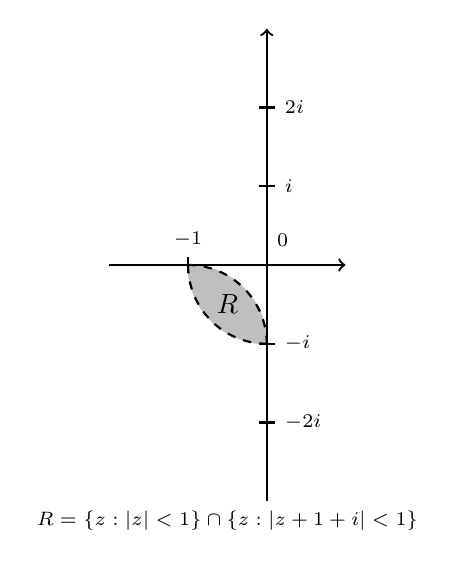
\begin{tikzpicture}
	% shading - must be drawn before the rest!
	\filldraw[color=lightgray] (-1,0) arc (0:90:-1) (0,-1) arc (0:90:1);
	\draw (-0.5,-0.5) node {$R$};
	% grid for draft only
	%%\draw [help lines] (-2,-3) grid (1,3);
	% legend
	\draw (-0.5,-3) node[below] {\scriptsize $R=\{z:|z|<1\} \cap \{z:|z+1+i|<1\}$};
	% the X-axis
	\draw[->,thick] (-2,0)--(1,0);
	\draw[thick] (-1,-0.1) -- (-1,0.1) node[above] {\scriptsize $-1$};
	\draw[thick] ( 0,-0.1) -- ( 0,0.1) node[above right] {\scriptsize $0$};
	% the Y-axis
	\draw[->,thick] (0,-3)--(0,3);
	\draw[thick] (-0.1,-1) -- (0.1,-1) node[right] {\scriptsize $-i$};
	\draw[thick] (-0.1,-2) -- (0.1,-2) node[right] {\scriptsize $-2i$};
	\draw[thick] (-0.1, 1) -- (0.1, 1) node[right] {\scriptsize $ i$};
	\draw[thick] (-0.1, 2) -- (0.1, 2) node[right] {\scriptsize $ 2i$};
	% inner circle border
	\draw[thick,style=dashed] (-1,0) arc (0:90:-1);
	% outer circle border
	\draw[thick,style=dashed] (0,-1) arc (0:90:1);
\end{tikzpicture}
%%\bigskip
%
%	The Region S
%
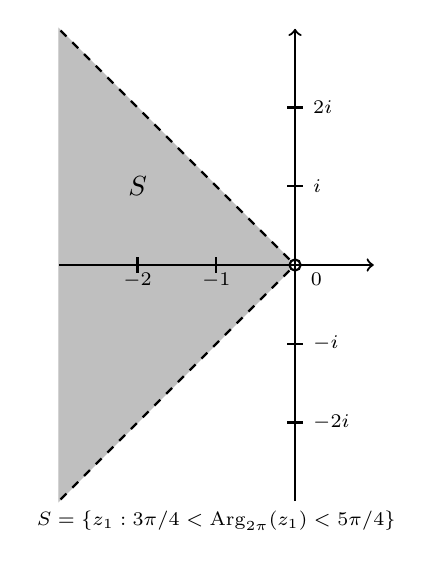
\begin{tikzpicture}
	% shading - must be drawn before the rest!
	\filldraw[color=lightgray] (-2pt,2pt) -- (-3,3) -- (-3,-3) -- (-2pt,-2pt);
	\draw (-2,1) node {$S$};
	% grid for draft only
	%%\draw [help lines] (-3,-3) grid (1,3);
	% legend
	\draw (-1,-3) node[below]
		{\scriptsize $S=\{z_1: 3\pi/4 < \Arg_{2\pi}(z_1) < 5\pi/4 \}$};
	% the X-axis
	\draw[->,thick] (-3,0)--(1,0);
	\draw[thick] (-2,-0.1) -- (-2,0.1) node[below=2pt] {\scriptsize $-2$};
	\draw[thick] (-1,-0.1) -- (-1,0.1) node[below=2pt] {\scriptsize $-1$};
	\draw[thick] ( 0,-0.1) -- ( 0,0.1) node[below right=2pt] {\scriptsize $0$};
	% the Y-axis
	\draw[->,thick] (0,-3)--(0,3);
	\draw[thick] (-0.1,-1) -- (0.1,-1) node[right] {\scriptsize $-i$};
	\draw[thick] (-0.1,-2) -- (0.1,-2) node[right] {\scriptsize $-2i$};
	\draw[thick] (-0.1, 1) -- (0.1, 1) node[right] {\scriptsize $ i$};
	\draw[thick] (-0.1, 2) -- (0.1, 2) node[right] {\scriptsize $ 2i$};
	% upper ray
	\draw[thick,style=dashed] (-2pt, 2pt) -- (-3,3);
	% lower ray
	\draw[thick,style=dashed] (-2pt,-2pt) -- (-3,-3);
	% exclude the origin
	\draw[thick] (0,0) circle(2pt);
\end{tikzpicture}

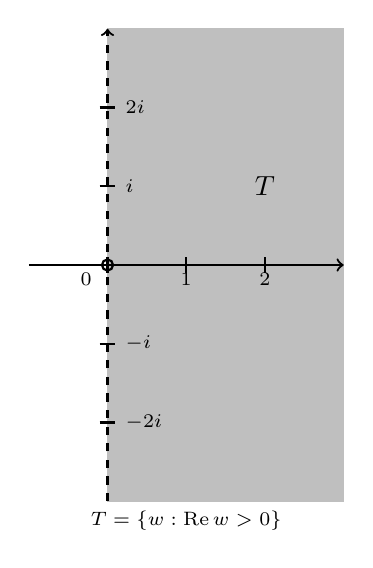
\begin{tikzpicture}
	% shading - must be drawn before the rest!
	\filldraw[color=lightgray] (0,3) -- (3,3) -- (3,-3) -- (0,-3) -- cycle;
	\draw (2,1) node {$T$};
	% grid for draft only
	%%\draw [help lines] (-1,-3) grid (3,3);
	% legend
	\draw (1,-3) node[below]
		{\scriptsize $T=\{ w: \RE\,w > 0 \} $};
	% the X-axis
	\draw[->,thick] (-1,0)--(3,0);
	\draw[thick] ( 2,-0.1) -- ( 2,0.1) node[below=2pt] {\scriptsize $ 2$};
	\draw[thick] ( 1,-0.1) -- ( 1,0.1) node[below=2pt] {\scriptsize $ 1$};
	\draw[thick] ( 0,-0.1) -- ( 0,0.1) node[below left=2pt] {\scriptsize $0$};
	% the Y-axis
	\draw[->,thick,style=dashed] (0,-3)--(0,3);
	\draw[thick] (-0.1,-1) -- (0.1,-1) node[right] {\scriptsize $-i$};
	\draw[thick] (-0.1,-2) -- (0.1,-2) node[right] {\scriptsize $-2i$};
	\draw[thick] (-0.1, 1) -- (0.1, 1) node[right] {\scriptsize $ i$};
	\draw[thick] (-0.1, 2) -- (0.1, 2) node[right] {\scriptsize $ 2i$};
	% exclude the origin
	\draw[thick] (0,0) circle(2pt);
\end{tikzpicture}


\item[(ii)]

The two boundaries (arcs) on $R$ map to the two boundaries (rays) in $S$.

$R$ is bounded, and $-i$ on $R$ is mapped to $\infty$ on $S$, which
is unbounded.

The angle of intersection of the arcs on $R$ at $-1$ is $\frac{\pi}{2}$,
this angle is preserved on the intersection of the two boundary rays of
$S$ at $0$.

The point $\infty$ is outside the bounded region $R$, this point is
mapped to $1$, which is also outside $S$

The point $\frac{1}{2}(-1-i)$ is in $R$, this point maps to $-1$, which
is in $S$.

Hence, $f$ is a conformal mapping from $R$ to $S$.

\item[(iii)]

We can map the region $S$ to the region $T$ with the square function,
$f_2(z_1)=z_1^2$, so $z_1\in S$ is mapped to $w\in T$.

Since the M\"{o}bius Transformation, $f_1$, is one-one and conformal
on $R$ and the square function, $f_2$, is one-one and conformal on $S$,
we can use their composite to map $R$ to $T$, $f = f_2 \circ f_1$, hence
\[
f(z) = f_2 ( f_1(z) ) = \left( \frac{ z+1 }{ z+i } \right)^2
\]
is a one-one conformal mapping from $R$ to $T$.

\item[(iv)]
For the inverse function we have $f^{-1} = f_1^{-1} \circ f_2^{-1}$,
where
\[
z_1 = f_2^{-1}(w) = -\sqrt{w}
\]
and\hbm{D1}{2.6}
\[
z = f_1^{-1}(z_1) = \frac{ iz_1 - 1 }{ -z_1 + 1 }
\]
Hence,
\[
z	= f^{-1}(w)
	= \frac{ i(-\sqrt{w}) - 1 }{ -(-\sqrt{w}) + 1 }
	= \frac{ -i\sqrt{w} - 1 }{ \sqrt{w} + 1 }
\]

\end{itemize}

\end{itemize}



\end{document}

